

\documentclass[12pt]{article}
\usepackage[T1]{fontenc}
\usepackage[utf8]{inputenc}
\usepackage{amsmath}
\usepackage{microtype}
\usepackage{listings}
\setlength{\parindent}{0pt}
\usepackage{fancyvrb}
\usepackage{enumerate}
\usepackage{array}
\usepackage[breaklinks=true,linktocpage,hidelinks]{hyperref}
\usepackage[letterpaper]{geometry}
\usepackage{url}
\usepackage{graphicx}
\usepackage{fullpage}

\usepackage{pgfplots}
\usepackage{pgfplotstable}
\usepackage{tikz}

\usepackage{fancyhdr}
\usepackage{fancybox}
\usepackage{multicol}
\usepackage{xcolor}
\usepackage{adjustbox}

\pgfplotsset{compat=newest}
\usetikzlibrary{shapes,backgrounds,arrows}
\usepgfplotslibrary{external} 

\definecolor{brewcol1}{RGB}{166,206,227}
\definecolor{brewcol2}{RGB}{31,120,180}
\definecolor{brewcol3}{RGB}{178,223,138}
\definecolor{brewcol4}{RGB}{51,160,44}
\definecolor{brewcol5}{RGB}{251,154,153}
\definecolor{brewcol6}{RGB}{227,26,28}
\definecolor{brewcol7}{RGB}{237,179,1}
\definecolor{brewcol8}{RGB}{202,178,214}
\definecolor{brewcol9}{RGB}{206,27,1}

\geometry{hmargin=1.87cm, vmargin=1.87cm}
\bibliographystyle{siam}

\DeclareTextFontCommand{\helvetica}{\fontfamily{phv}\selectfont\small}


\begin{document}

\clearpage\thispagestyle{empty}
\begin{center}
\textbf{Difficult transition for sugar maple in Boreal forest under climate change? \\
Impact of alternative stable states on Sugar maple migration.}
\vskip 2em
Research proposal
\vskip 1em
Master in Wildlife management
\vfill
By
\vfill
Steve Vissault 
\vfill 
For
\vfill
\textbf{Richard Cloutier}, Pr.\\
Director of the program committee
\vskip 2em
\textbf{Dominique Arsenault}, Pr.\\
President of the jury
\vskip 2em
\textbf{Matt Talluto}, PhD\\
Research Co-director
\vskip 2em
\textbf{Dominique Gravel}, Pr.\\
Research Director
\vfill
\vfill
Université du Québec à Rimouski\\
\today

\end{center}

\newpage
\setcounter{page}{1}

\section{Introduction}

\textbf{Context.}  The boreal region is warming twice as fast as the global
average and will inevitably alter species composition in boreal forest
\cite{Scheffer2012,Hughes2000}.  Sugar maple is one of those species expected
to migrate northward towards it's nordic temperate forest limits
\cite{McKENNEY2007,Goldblum2005}. Predict shifts in the repartition of sugar
maple under climate change is an important challenge whereas this species is
highly coveted by hardwood and maple syrup producers, two main economic
sectors in Quebec. Indeed, Sugar maple is a widespread and abundant tree in
north-eastern North America and one of the most representative species of
northern temperate forests \cite{Graignic2013,Messaoud2007,Kellman2004}. This
northward migration will result in increasing the surface of the ecotone
between the boreal and temperate forest of Quebec. Nevertheless, the expansion
of species distribution occuring in Nordic temperate forest could be difficult
and explain by the fact than microclimatic conditions found in boreal forests
are different from those present in temperate forest. Colder temperatures from
shading and excess soil moisture due to snow melt cause litter to be more
acidic and fibrous during the spring. Therefore, even if the regional climate
conditions are favorable \cite{Kellman2004}, the microbiota conditions found
in the boreal forest could affect the establishment of sugar
maple\cite{Kellman2004,Moore2008,DeFrenne2013}. In this case, the sugar maple
could be unable to migrate in boreal forests as a result of negative soil
feedback (\textbf{$H_0$}). This phenomen could increase the tension between
the boreal forest and the nordic temperate forest and generating abrupt
changes in the community composition.\\

This project aim to develop a state and transition model (STM) between the
boreal and temperate nordic forest in order to investigate on the shift in the
distribution of sugar maple into the boreal-temperate forest dynamical system.
To realized this objective, we will use the alternative stable states theory
as a framework. The first section aims to present the main objectives of this
master project. In order to define the context of this study, the second
section is a review subdivided into two paragraphs. The first part will
present the theorical context on the alternative stable states and abrupt
changes in ecosystems functionning. Second part of this section will focus on
the Sugar maple and his community and thus explain why is alternative stable
states a relevant framework to study the dynamic of the boreal-temperate
forests ecotone.  The third section of this document will describe the model
and the methodology employed to assess the objectives. To conclude, the last
part will present the general timeline associated to this project.

\section{Objectives} 

This project aims to determine whether alternative stable states are present
in the temperate-boreal forest ecotone and if so, look at the impact of plant-
soil and disturbances feedback on the alternatives stables states. To assess
this main objective, we will (1) generate a transitional model between the
temperate and the boreal forest; (2) investigate the spatial structure of the
transitonnal zone; and finaly (3) run simulations based on different climate
change scenarios.

%% See with Matt about linked the model with the main hypothesis

\section{Review} 

\textbf{Theorical framework.}  Many ecotone studies and modeling efforts on
transition between forest to none-forest ecosystems (e. i. Boreal - Toundra)
\cite{Scheffer2012,Scheffer2001,Hirota2011} but little attention has been
given to evaluate the transitional dynamics of forest-forest ecotone
\cite{Goldblum2010,Graignic2013}. At large scale, transition between  the
temperate nordic and the boreal forests can be approach as a dynamic system
where each forest biomes is a state. The presence of different states at a
location or a time depends on environmental conditions (e. i. Soil,
temperature) encountered by the system. When small environnemental
fluctuations occurs, mostly dynamical system can respond almost linearly with
no particular threshold to observe drastic changes in state of the ecosystem (
Figure \ref{fig1} .A)} \cite{Scheffer2001,Scheffer2009}. Thus, increase the
soil moisture might cause favorable conditions to a new species, but doesn't
affect the functionning of the ecosystem. In this case, only one equilibrium
can be observed given a specific environnemental condition
\cite{Scheffer2001,Scheffer2009,scheffer2009critical}. Another kind of
system response occurs more frequently in nature.  Natural systems are rather
insensitive over certain ranges of environnementals conditions while
responding strongly when a treshold is reached by the system
\cite{scheffer2009critical}.  As example, Scheffer \citep{scheffer2009critical} \\

% Ouvrir pour le prochain paragraph avec Goldblum p.703

\textbf{Natural system.}  

Partir sur les principaux facteurs drivant la dynamique d'un écotone
Détailler les communautés;
Justifier le choix des espèces; 
Reprendre l'anayse préliminaire sur les ALSST et 


% We used maple sugar basa areal in function of black
% spruce, white spruce and balsam fir basal area to compute the relative
% abundance of sugar maple. Given the above statements, we used mainly two
% climatic variables (annual mean temperature and annual precipitation) to
% identify the alternative stable states present in the boreal-temperate
% ecotone. The relationship was performed on climatic variables and sugar maple
% relative abundance using kernel density plot function. We obtained the
% probability of observed a sample plot as function of sugar maple relative
% abundance and mean annual temperature (Figure \ref{fig1}). In both case,
% alternative stable states are presents whereas the function graphed has a
% bimodal distribution. At low precipitation or temperature conditions, the
% probability of observing a parcel sampled without sugar maple is higher than
% intermediate climatic conditions where the multimodal distribution appear. The
% density function suggest the presence of alternative stabe states  in response
% of intermediate climatic conditions: one state wherein sugar maple dominates
% and an another in which sugar maple is absent. \\


\begin{figure}[ht]       
\begin{center}
	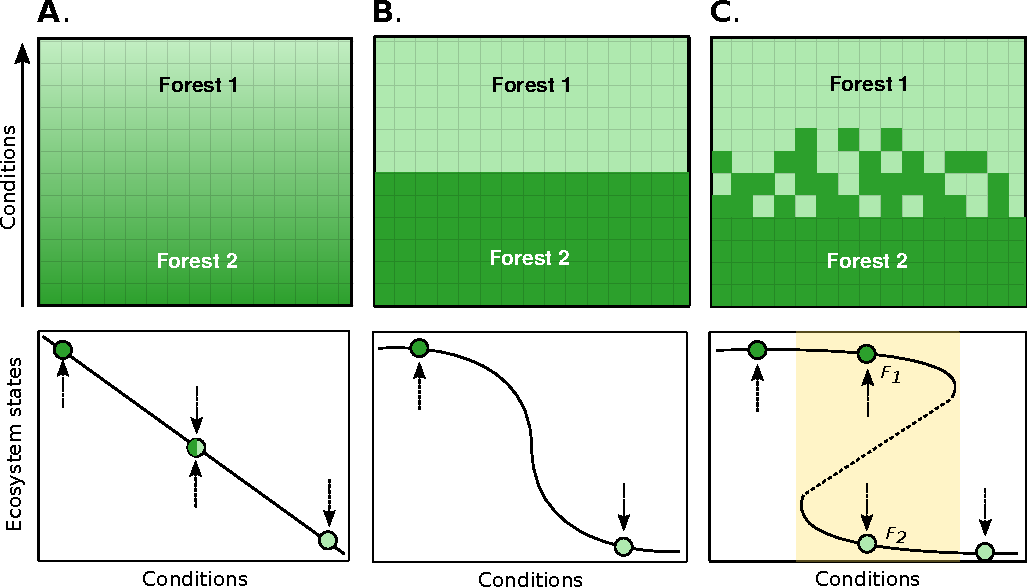
\includegraphics[width=\textwidth]{fig/states.pdf}       
\end{center}
\caption{Schematic representation of different ways in which the equilibrium
state of a system can vary with conditions such as temperature, precipitation
or soil moisture. Three differents kinds of respond are presented,
\textbf{(A)} gradual, \textbf{(B)} basic fold, \textbf{(C}) catastrophic fold.
The first panels line is a conceptualization of a transitional landscape
between the boreal (light green) and the nordic temperate forests (dark
green). The second panels line presents the stable states rise by the forest
given a specific environnemental condition. Each arrows in graphs indicate the
point toward the system moves if it's not at the equilibrium. Every point on
the plain line could be a stable state encounter by the boreal-temperate
forests system, excepted for the dashed line (in yellow highlight). This zone,
called hysteresis, are particulary unstable and little fluctuations in
environnement conditions give rise to a contrasted state representing an
alternative stable states.  ($F_1$ or $F_2$).}

% Manque le rapprochement avec la première ligne

\label{fig1}
\end{figure}

\section{Methods}   

\textbf{Models.} This state and transition model will be based on four
differents states: \textbf{(D)} Decidious; \textbf{(C)} Coniferious;
\textbf{(M)} Mixed stand and finaly \textbf{(T)} Transitional stand. Whereas
parameters previously announced, this model can be formally describe by this
set of differential equations:


\begin{equation}
	\begin{align*}
	\frac{dE}{dt} &= E - E \cdot (P_C +P_D - P_M) \\
	\frac{dS}{dt} &= P_M\cdot E + bC\cdot (C+M)\cdot D + \beta_D\cdot (D+M)\cdot C - S_C\cdot M -S_D\cdot M - e\cdot M \\
	\frac{dS}{dt} &=
	\end{align*}
\end{equation}
%dEdt = E - E\cdot (pC + pD - pM) 
%dMdt = pM\cdot E + bC\cdot (C+M)\cdot D + bD\cdot (D+M)\cdot C - sC\cdot M - sD\cdot M - e\cdot M
%dCdt = pC_\cdot E + sC\cdot M - bD\cdot (D+M)\cdot C - e\cdot C
%dDdt = pD_\cdot E + sD\cdot M - bC\cdot (C+M)\cdot D - e\cdot D



\begin{center}
	
				\tikzstyle{noeud}=[circle,
				                  thick,
				                  minimum size = 1.5cm,
				                  inner sep =5pt,
				                  draw=brewforest3,
				                  fill=brewforest1]
				\tikzstyle{noeud2}=[circle,
				                  thick,
				                  minimum size = 1.5cm,
				                  inner sep =5pt,
				                  draw=brewforest3,
				                  fill=brewforest3]
				\tikzstyle{noeud3}=[circle,
				                  thick,
				                  minimum size = 1.5cm,
				                  inner sep =5pt,
				                  draw=brewforest3,
				                  fill=brewforest3]
	
				\begin{tikzpicture}[->,>=stealth',auto,scale=0.65]
				      \node [circle,noeud2] (M) at (0,0) {\color{white}\textbf{M}};
				      \node [circle,noeud2]  (C) at (-5,5) {\color{white}\textbf{C}};
				      \node [circle,noeud2] (D) at (5,5) {\color{white}\textbf{D}};
				      \node [circle,noeud2] (T) at (0,10) {\color{white}\textbf{T}};
	
						\draw[thick,-latex] (M) to[bend right=10] node[above,sloped] {$S_C$} (C);
						\draw[thick,-latex] (C) to[bend right=10] node[below,sloped] {$\beta_d \cdot (D+M)$} (M);
	
						\draw[thick,-latex] (D) to[bend right=10] node[above,sloped] {$\beta_c \cdot (C+M)$} (M);
						\draw[thick,-latex] (M) to[bend right=10] node[below,sloped] {$S_D$} (D);
	
						\draw[thick,-latex] (D) to[bend right=10] node[above,sloped] {$e$} (T);
						\draw[thick,-latex] (T) to[bend right=10] node[below,sloped] {$\phi_D$} (D);
	
						\draw[thick,-latex] (T) to[bend right=10] node[above,sloped] {$\phi_C$} (C);
						\draw[thick,-latex] (C) to[bend right=10] node[below,sloped] {$e$} (T);
	
						\draw[thick,-latex,transform canvas={xshift=0.8ex}] (T) to node[above,sloped,rotate=90,transform canvas={xshift=3ex}] {$\phi_M $} (M);
						\draw[thick,-latex,transform canvas={xshift=-0.8ex}] (M) to node[above,sloped,rotate=-90,transform canvas={xshift=-3ex}] {$e$} (T);
				\end{tikzpicture}
	\end{center}	



%- Générale description du model (États et paramètre)
%- Description des transition entres les états (approcher par équations différentielles)
%- Justifier la pertinence des paramètres choisis
%- Justifier les postulats. Certaines espèces ne participent pas à la transition et pourquoi ? 
%- Monter la technique de validation de la classification en fonction des observations 


\textbf{Paramerization.} The parameterization of this model will be
conducted on the QUICC-FOR database containing large permanent sample plots
surveys. Those data are provided by several forest offices and cover multiple
canadian provinces ($\pm16 000$ plots) and states (\textbf{Ask at Miranda} plots).
These inventories started since the 1970s and include all stems measurements
and forest stand informations relative to a specific plot location and year. In a first
time, the basal area will be compute to provide a measure of relative growth
of each species present in the plots. \\

\textbf{Validation.}

- Matrice de confusion sur la classification des patchs (M,D,C,T)
- Matrice de confusion (TSS) et AUC sur un jeux de données indépendants 
- Spatialement explicit à l'aide de l'automate cellulaire.

\textbf{Simulation.}

This model will be incorporated in a spatially explicit cellular automata in
order to evaluate the transition rate of those patches under differents
climate change scenario.

- Temps discrets
- Cellulaire automate

\newpage
\bibliography{/home/steve/Dropbox/Bibtex/Devis}
\end{document}
